\documentclass{beamer}
\usepackage[utf8]{inputenc}
\usepackage{amsmath}
\usepackage{amssymb}
\usepackage{graphicx}
\usepackage{booktabs}
\usepackage{xcolor}
\usepackage{colortbl}
\usepackage{algorithm}
\usepackage{algpseudocode}
\algrenewcommand\algorithmicindent{0.8em}
\usetheme{CambridgeUS}
\usecolortheme{beaver}

\definecolor{darkred}{RGB}{180,30,30}
\definecolor{lightgray}{RGB}{240,240,240}
\definecolor{hlblue}{RGB}{220,235,255}

\setbeamertemplate{blocks}[rounded][shadow=true]
\setbeamertemplate{itemize item}{\textbullet}
\setbeamertemplate{itemize subitem}{--}
\setlength{\leftmargini}{1.2em}

\setbeamertemplate{footline}{%
  \leavevmode%
  \hbox{%
    \begin{beamercolorbox}[wd=.40\paperwidth,ht=2.25ex,dp=1ex,center]{author in head/foot}%
      \usebeamerfont{author in head/foot}\insertshortauthor
    \end{beamercolorbox}%
    \begin{beamercolorbox}[wd=.40\paperwidth,ht=2.25ex,dp=1ex,center]{title in head/foot}%
      \usebeamerfont{title in head/foot}\insertshorttitle
    \end{beamercolorbox}%
    \begin{beamercolorbox}[wd=.20\paperwidth,ht=2.25ex,dp=1ex,right]{date in head/foot}%
      \insertframenumber{} / \inserttotalframenumber\hspace*{2ex}
    \end{beamercolorbox}%
  }%
  \vskip0pt%
}

\title[Aerodrome Race Optimisation]{Aerodrome Race Optimisation}
\author[DIN Sokheng]{DIN Sokheng}
\institute{ENSIIE --- Universit\'e Paris-Saclay}
\date{CORO Project \,--\, 2025--2026}

\newcommand{\hrow}{\rowcolor{hlblue}}

\begin{document}

\maketitle

% ================================================================
\begin{frame}{Problem Statement}

\begin{block}{\textbf{Input}}
\small
$n$ aerodromes with coordinates $(x_i, y_i)$, region $r_i \in \{0,\ldots,m\}$,
start $s$, end $t$, minimum visits $V_{\min}$, range $R$.
Distances: $d(i,j) = \mathrm{round}\!\left(\sqrt{(x_i-x_j)^2+(y_i-y_j)^2}\right)$.
\end{block}

\begin{block}{\textbf{Objective}}
\small
Find path $s = v_1 \to \cdots \to v_k = t$ minimising
$\displaystyle\sum_{\ell=1}^{k-1} d(v_\ell, v_{\ell+1})$ subject to:
\begin{itemize}\setlength\itemsep{2pt}
  \item $d(v_\ell, v_{\ell+1}) \leq R$ \quad (range constraint)
  \item Each region $\kappa=1,\ldots,m$ has at least one visited aerodrome \quad (coverage)
  \item $k \geq V_{\min}$ \quad (minimum visits)
\end{itemize}
\end{block}

\begin{block}{\textbf{Difference from TSP}}
\small
\begin{itemize}\setlength\itemsep{2pt}
  \item Path from $s$ to $t$, not a Hamiltonian cycle
  \item Subset selection: we choose which aerodromes to visit
  \item Region-covering adds a set-covering structure
  \item Range constraint creates a sparse directed graph
\end{itemize}
\end{block}

\end{frame}

% ================================================================
\begin{frame}{Graph Construction}

\begin{columns}[T]
\begin{column}{0.50\textwidth}
\begin{block}{\textbf{Arc set}}
\small
Build directed graph $G=(V,A)$:
$$A = \{(i,j) : i \neq j,\; d(i,j) \leq R\}$$
Arcs violating range do not exist.\\[4pt]
Reduces variables from $n(n{-}1)$ to $|A|$.
\end{block}

\vspace{4pt}

\begin{block}{\textbf{Example: \texttt{instance\_6\_1}}}
\small
$n=6$, $s=1$, $t=5$, $V_{\min}=4$, $m=2$, $R=6$\\[3pt]
$d(1,3)=3 \leq 6$ \checkmark \quad
$d(3,2)=4 \leq 6$ \checkmark\\
$d(2,5)=5 \leq 6$ \checkmark \quad
$d(1,2)=7 > 6$ \texttimes\\[3pt]
\textbf{24 arcs} within range.\\
Optimal: $1 \to 3 \to 2 \to 5$, cost $= 12$.
\end{block}
\end{column}

\begin{column}{0.48\textwidth}
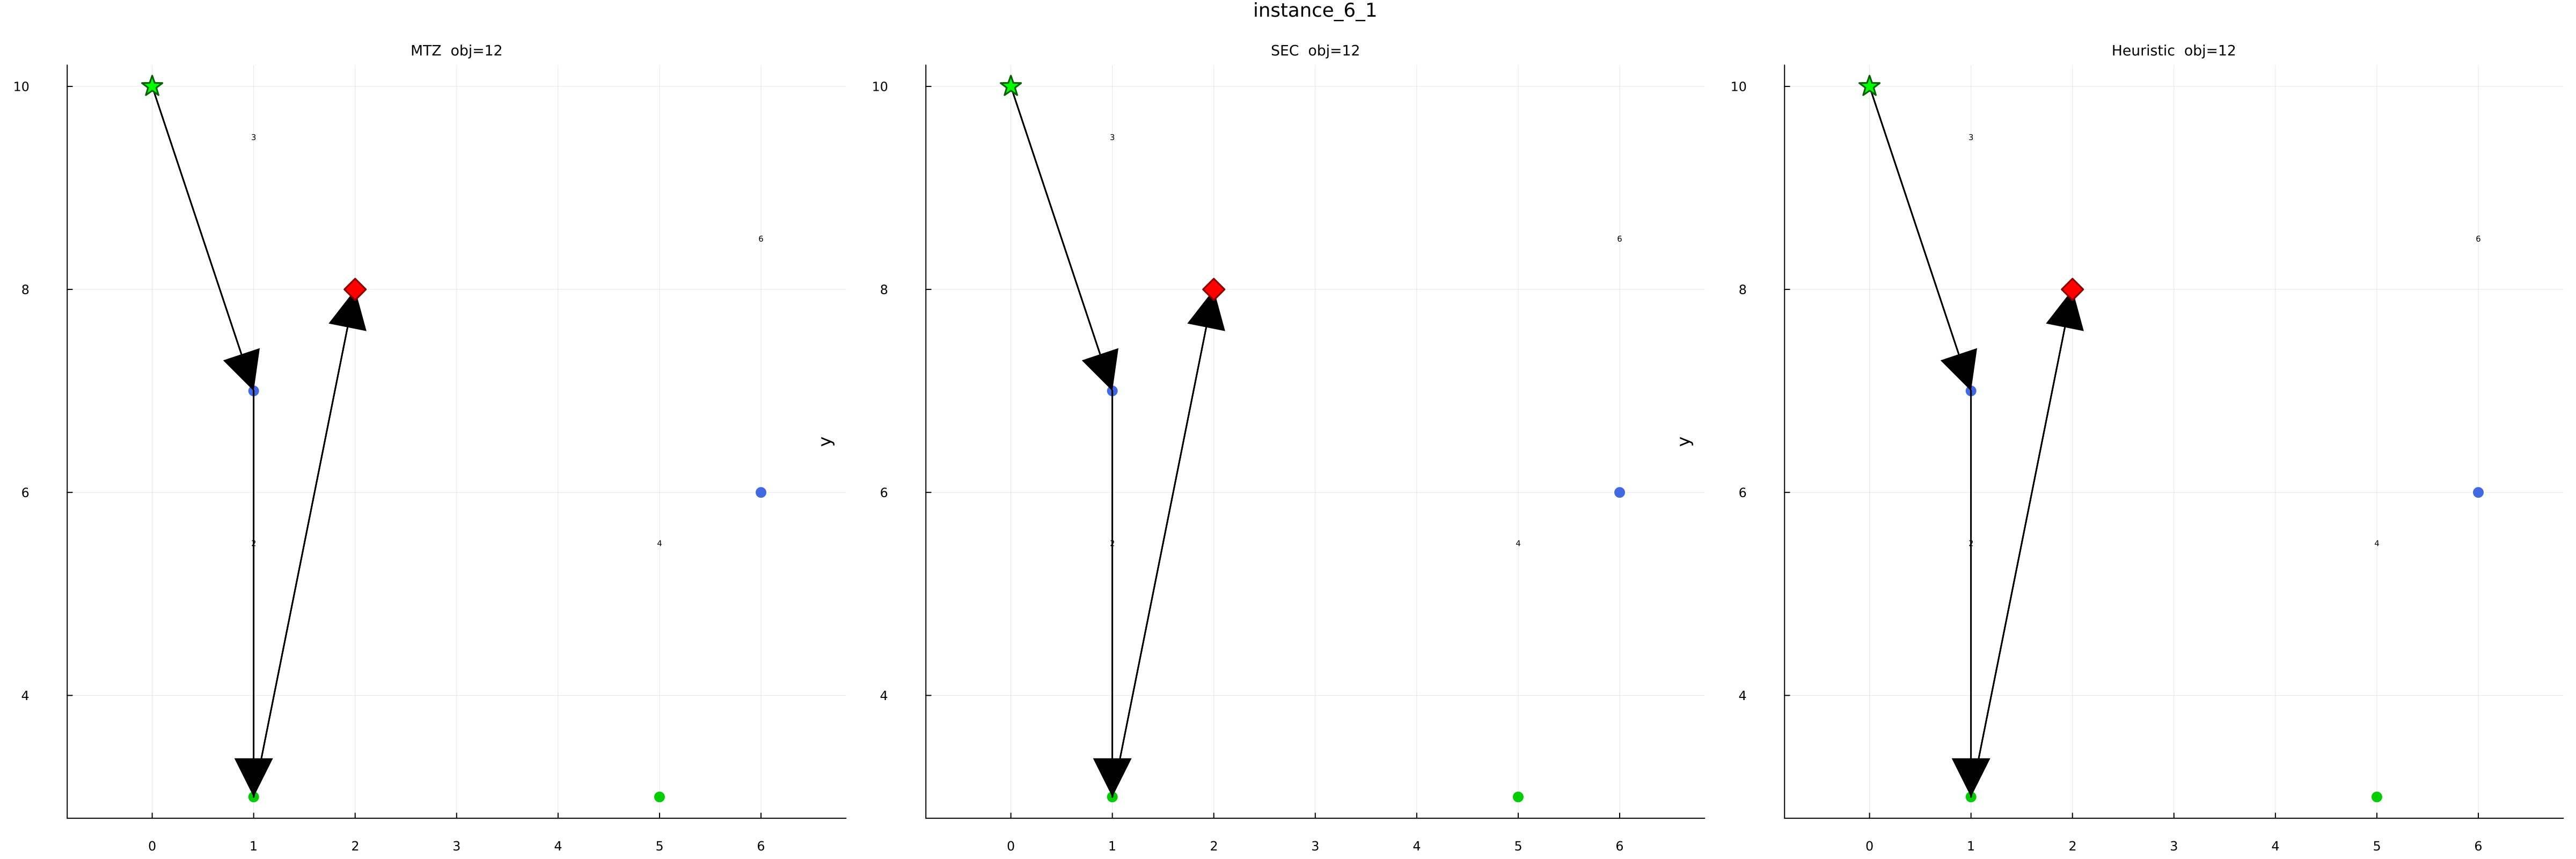
\includegraphics[width=\textwidth]{instance_6_1_results.png}
\end{column}
\end{columns}

\end{frame}

% ================================================================
\begin{frame}{ILP Model 1 --- MTZ Formulation}

\begin{columns}[T]
\begin{column}{0.50\textwidth}
\begin{block}{\textbf{Variables}}
\small
\begin{itemize}\setlength\itemsep{1pt}
  \item $x_{ij}\in\{0,1\}$: arc $(i,j)$ used
  \item $y_i\in\{0,1\}$: aerodrome $i$ visited
  \item $u_i\in[0,n]$: position along path
\end{itemize}
\end{block}

\vspace{4pt}

\begin{block}{\textbf{Key constraints}}
\small
\textbf{C1--C4:} flow conservation at $s$, $t$, intermediate nodes, force $y_s=y_t=1$.\\[3pt]
\textbf{C5:} $\sum_{i:\,r_i=\kappa} y_i \geq 1$ \quad for each region $\kappa$\\[3pt]
\textbf{C6:} $\sum_i y_i \geq V_{\min}$\\[3pt]
\textbf{C7 (MTZ):} for $(i,j)\in A$, $i\neq s$, $j\neq s$:
$$u_i - u_j + n\,x_{ij} \leq n-1$$
\textbf{C8:} $u_s=0$; $u_i \leq n\cdot y_i$
\end{block}
\end{column}

\begin{column}{0.48\textwidth}
\begin{block}{\textbf{MTZ solve (pseudocode)}}
\footnotesize
\begin{algorithmic}[1]
\State Build ILP with $x_{ij}$, $y_i$, $u_i$, constraints C1--C8.
\State Solve LP relaxation $\Rightarrow z_{\mathrm{LP}}$ (lower bound).
\If{LP solution is integer} \State \Return it. \EndIf
\Repeat
  \State Branch on most fractional $x_{ij}$.
  \State Solve LP at B\&B node.
  \If{infeasible} \State \textbf{prune}. \EndIf
  \If{bound $\geq z^*$} \State \textbf{prune}. \EndIf
  \If{integer \& better} \State update $z^*$. \EndIf
\Until{queue empty}
\State \Return best solution $z^*$.
\end{algorithmic}
\end{block}

\vspace{2pt}

{\footnotesize $O(n^2)$ constraints. \textcolor{darkred}{Weak LP relaxation} $\Rightarrow$ more B\&B nodes.}
\end{column}
\end{columns}

\end{frame}

% ================================================================
\begin{frame}{ILP Model 2 --- Subtour Elimination Constraints}

\begin{columns}[T]
\begin{column}{0.50\textwidth}
\begin{block}{\textbf{Same variables, no $u_i$}}
\small
Replace C7--C8 with SEC.\\
For every $\emptyset \neq S \subseteq V\setminus\{s,t\}$:
$$\sum_{\substack{(i,j)\in A\\i\in S,\,j\in S}} x_{ij} \leq |S|-1$$
Among $|S|$ nodes, any acyclic subgraph has $\leq |S|-1$ arcs.
If $\geq |S|$ arcs exist inside $S$, a disconnected cycle exists.
\end{block}

\vspace{4pt}

\begin{block}{\textbf{Iterative solve-and-cut}}
\footnotesize
\begin{algorithmic}[1]
\State Solve ILP with C1--C6 only.
\Repeat
  \State BFS from $s$ on used arcs.
  \State $U \leftarrow \{i : y_i=1,\; i \text{ unreachable from } s\}$
  \If{$U = \emptyset$} \State \Return current solution. \EndIf
  \For{each component $S$ of $U$}
    \State Add: $\sum_{i,j\in S} x_{ij} \leq |S|-1$
  \EndFor
  \State Re-solve ILP.
\Until{valid}
\end{algorithmic}
\end{block}
\end{column}

\begin{column}{0.48\textwidth}
\begin{block}{\textbf{LP relaxation quality}}
\small
$$z_{\mathrm{LP}}^{\mathrm{SEC}} \;\geq\; z_{\mathrm{LP}}^{\mathrm{MTZ}} \;\geq\; z_{\mathrm{ILP}}^*$$
SEC describes the subtour polytope exactly.\\[4pt]
Tighter LP bound $\Rightarrow$ fewer B\&B nodes pruned.
\end{block}

\vspace{4pt}

\begin{block}{\textbf{Tradeoff}}
\small
\begin{itemize}\setlength\itemsep{2pt}
  \item $2^{n-2}$ possible SEC constraints
  \item Separation: BFS in $O(n+|A|)$
  \item Our iterative approach re-solves from scratch at each iteration \textcolor{darkred}{(overhead)}
  \item Lazy callbacks would preserve the B\&B tree
\end{itemize}
\end{block}
\end{column}
\end{columns}

\end{frame}

% ================================================================
\begin{frame}{Heuristic --- Three Phases}

\begin{columns}[T]
\begin{column}{0.48\textwidth}
\begin{block}{\textbf{Phase 1: Greedy Construction}}
\footnotesize
\begin{algorithmic}[1]
\State $v\leftarrow s$; path $\leftarrow [s]$
\While{regions not all covered or $|\text{visited}|<V_{\min}$}
  \State $N\leftarrow$ unvisited neighbours of $v$ within $R$
  \If{$N=\emptyset$} \State Dijkstra escape. \EndIf
  \State Prefer $j\in N$ in uncovered region; else nearest $j\in N$
  \State Append $j$; $v\leftarrow j$
\EndWhile
\State Append $t$ (direct or via Dijkstra).
\end{algorithmic}
\end{block}

\vspace{3pt}

\begin{block}{\textbf{Phase 2: 2-opt}}
\footnotesize
\begin{algorithmic}[1]
\Repeat
  \For{all pairs $i<j$ (interior)}
    \State Reverse $[v_i,\ldots,v_j]$; accept if $d\leq R$ and shorter.
  \EndFor
\Until{no improvement}
\end{algorithmic}
\end{block}
\end{column}

\begin{column}{0.48\textwidth}
\begin{block}{\textbf{Phase 3: Node Removal}}
\footnotesize
\begin{algorithmic}[1]
\Repeat
  \State Find $v_\ell$ maximising saving s.t.
  \State \hspace{1em} $d(v_{\ell-1},v_{\ell+1})\leq R$,\; $|\text{path}|-1\geq V_{\min}$
  \State \hspace{1em} region $r_{v_\ell}$ covered by another node
  \If{found} \State Remove $v_\ell$. \EndIf
\Until{none removable}
\end{algorithmic}
\end{block}

\vspace{4pt}

\begin{block}{\textbf{Known limitation}}
\small
On sparse graphs ($R$ tight), the Dijkstra escape skips already-visited intermediate hops to avoid duplicates, leaving direct connections that were never checked for range feasibility $\Rightarrow$ infeasible legs on large instances.
\end{block}
\end{column}
\end{columns}

\end{frame}

% ================================================================
\begin{frame}{Results --- Small Instance (\texttt{instance\_6\_1})}

\begin{columns}[T]
\begin{column}{0.45\textwidth}
\renewcommand{\arraystretch}{1.3}
\small
\begin{tabular}{lrrr}
\toprule
\textbf{Method} & \textbf{Obj.} & \textbf{Time (s)} & \textbf{B\&B} \\
\midrule
\hrow MTZ       & \textbf{12} & 0.09  & 1 \\
SEC             & \textbf{12} & 0.02  & 1 \\
\hrow Heuristic & \textbf{12} & 0.12  & --- \\
\bottomrule
\end{tabular}

\vspace{6pt}
\small
All three find optimal path $1\to3\to2\to5$, cost $=12$.\\[4pt]
Both ILP models solve at root node (1 B\&B node, no branching).\\[4pt]
SEC added 3 cuts before converging.\\[4pt]
Heuristic matches the optimum exactly.
\end{column}

\begin{column}{0.52\textwidth}
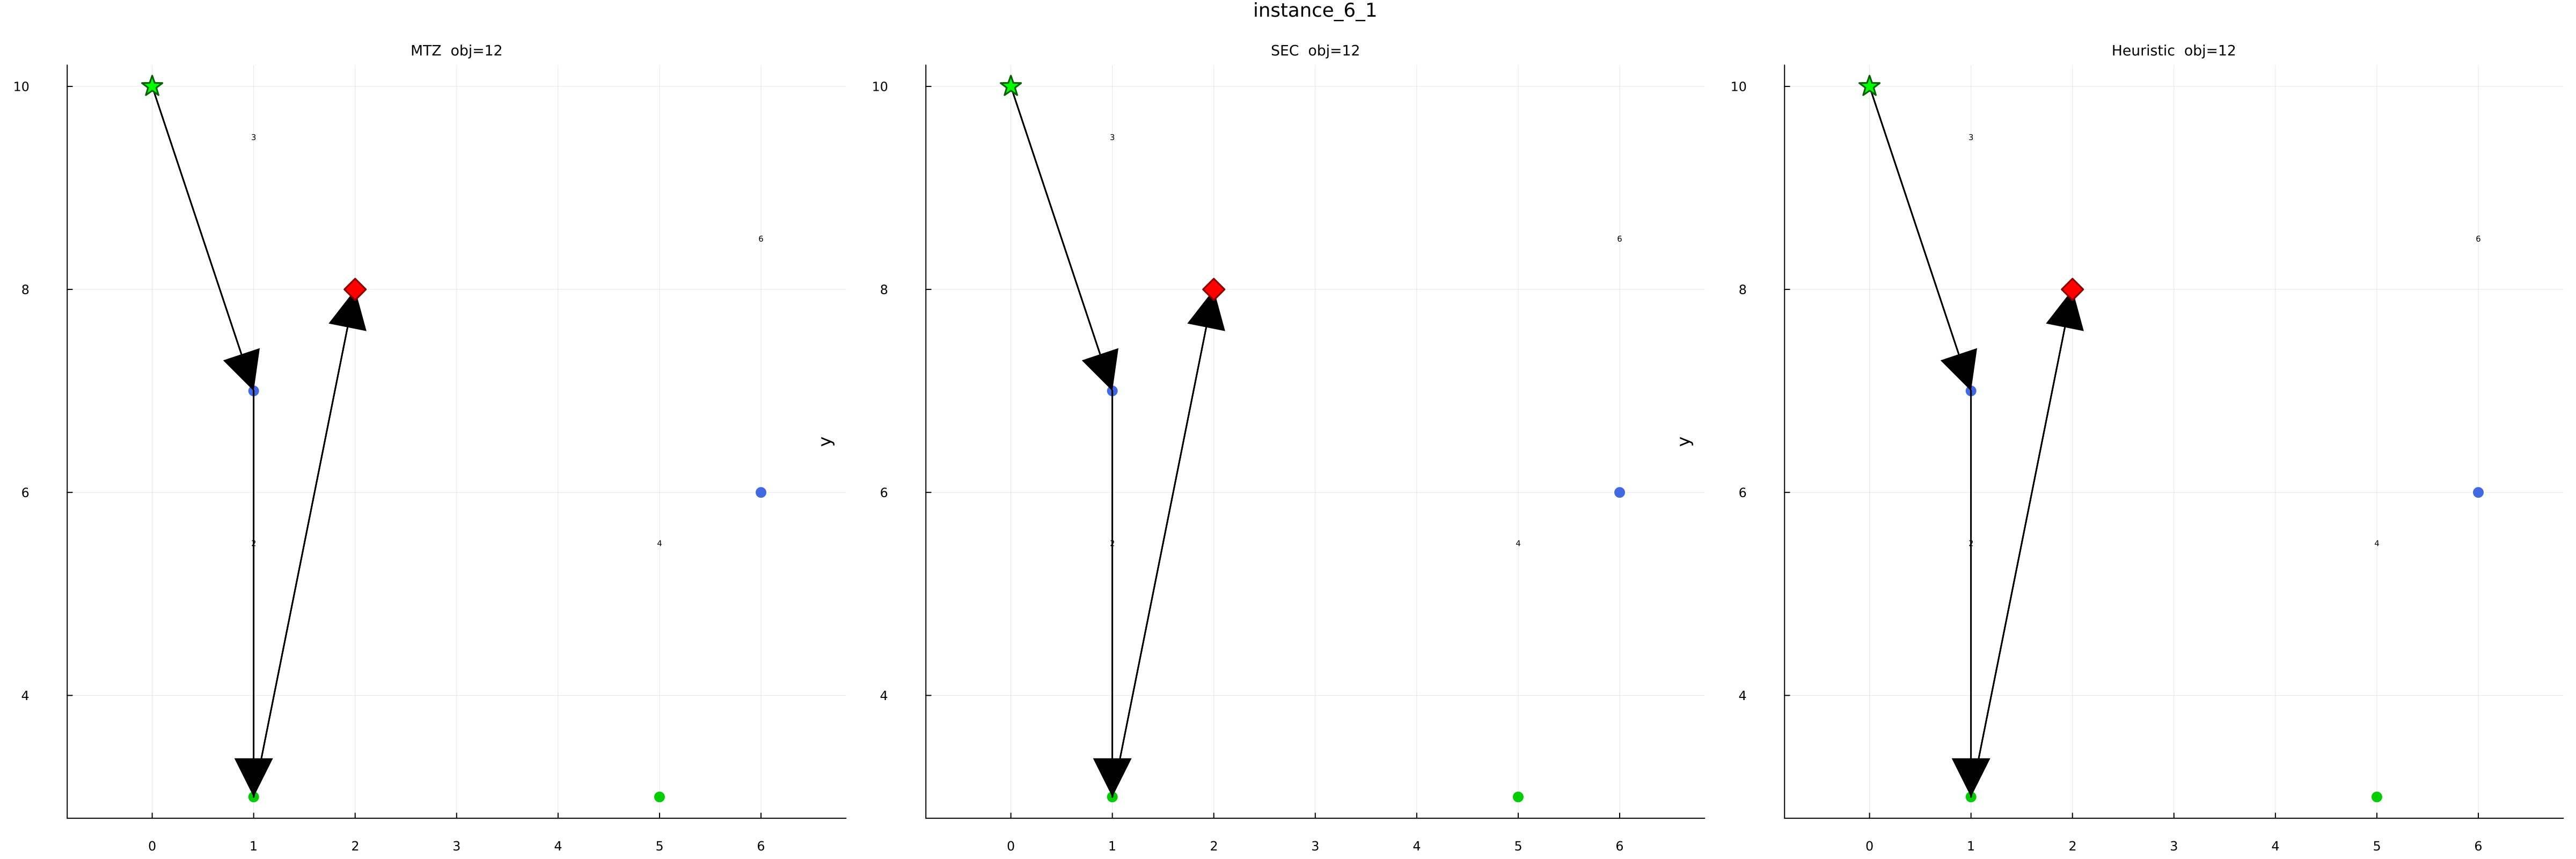
\includegraphics[width=\textwidth]{instance_6_1_results.png}
\end{column}
\end{columns}

\end{frame}

% ================================================================
\begin{frame}{Results --- Medium Instance (\texttt{instance\_40\_1})}

\begin{columns}[T]
\begin{column}{0.45\textwidth}
\renewcommand{\arraystretch}{1.3}
\small
\begin{tabular}{lrrr}
\toprule
\textbf{Method} & \textbf{Obj.} & \textbf{Time (s)} & \textbf{B\&B} \\
\midrule
\hrow MTZ       & \textbf{114} & 4.63   & 1\,295 \\
SEC             & \textbf{114} & 35.38  & 35 \\
\hrow Heuristic & 155          & $<$0.01 & --- \\
\bottomrule
\end{tabular}

\vspace{4pt}
\small
Both ILP models prove optimal cost 114.\\[3pt]
SEC uses $37\times$ fewer B\&B nodes (35 vs.\ 1\,295) --- tighter LP bound confirmed.\\[3pt]
MTZ is $8\times$ faster: iterative SEC discards the B\&B tree after each cut batch (66 cuts total).\\[3pt]
Heuristic gap: $+35.96\%$.
\end{column}

\begin{column}{0.52\textwidth}
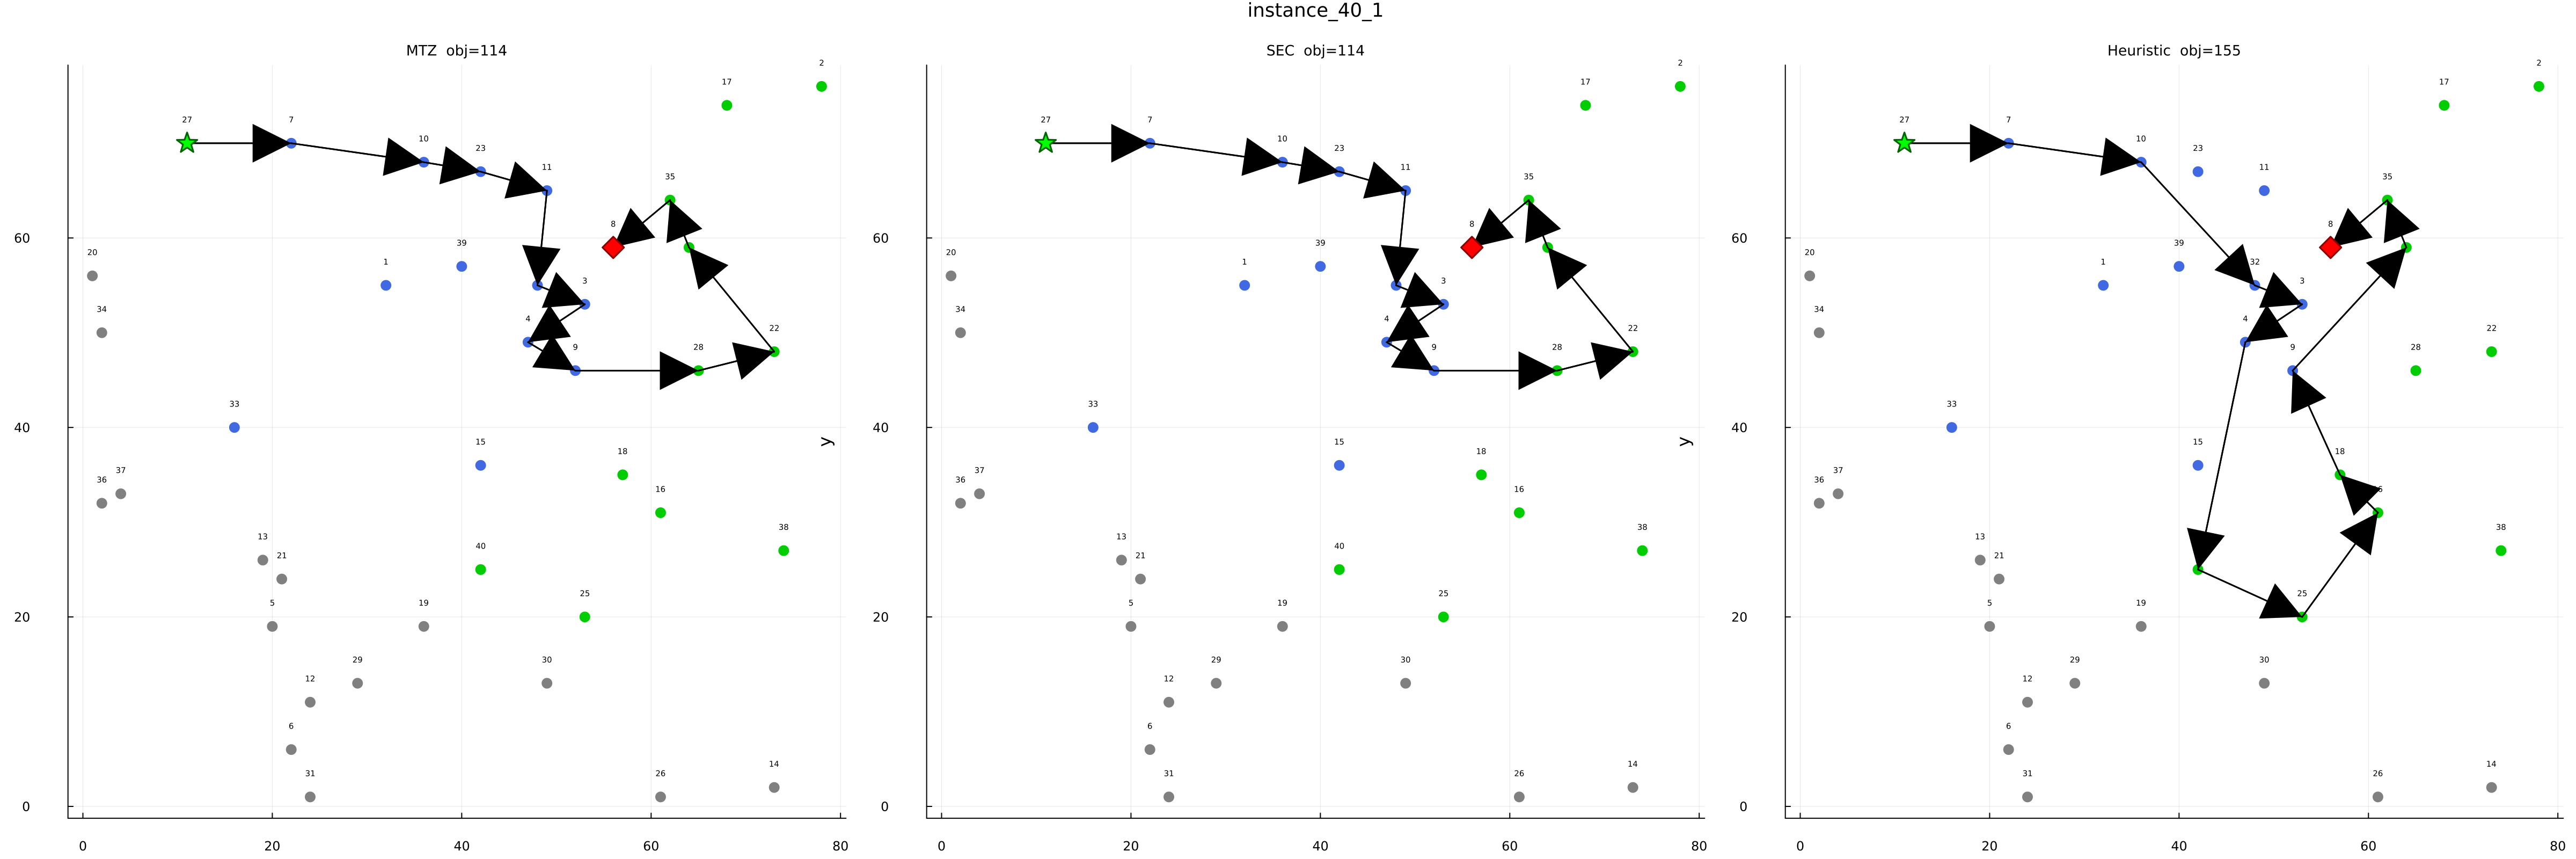
\includegraphics[width=\textwidth]{instance_40_1_results.png}
\end{column}
\end{columns}

\end{frame}

% ================================================================
\begin{frame}{Results --- Large Instance (\texttt{instance\_80\_1})}

\begin{columns}[T]
\begin{column}{0.45\textwidth}
\renewcommand{\arraystretch}{1.3}
\small
\begin{tabular}{lrrl}
\toprule
\textbf{Method} & \textbf{Obj.} & \textbf{Time (s)} & \textbf{Status} \\
\midrule
\hrow MTZ       & 948 & 120.01 & Time limit \\
SEC             & --- & 165.41 & Time limit \\
\hrow Heuristic & 637 & $<$0.01 & Invalid\,$^\dagger$ \\
\bottomrule
\end{tabular}

\vspace{4pt}
\small $^\dagger$ Heuristic leg $19\to55$: dist $= 56 > R = 31$.\\[4pt]
MTZ found incumbent 948 (49 stops, 53\,334 nodes) but could not prove optimality.\\[4pt]
SEC added 105 cuts but found no valid solution within 165\,s.\\[4pt]
Each SEC re-solve consumed part of the time budget.
\end{column}

\begin{column}{0.52\textwidth}
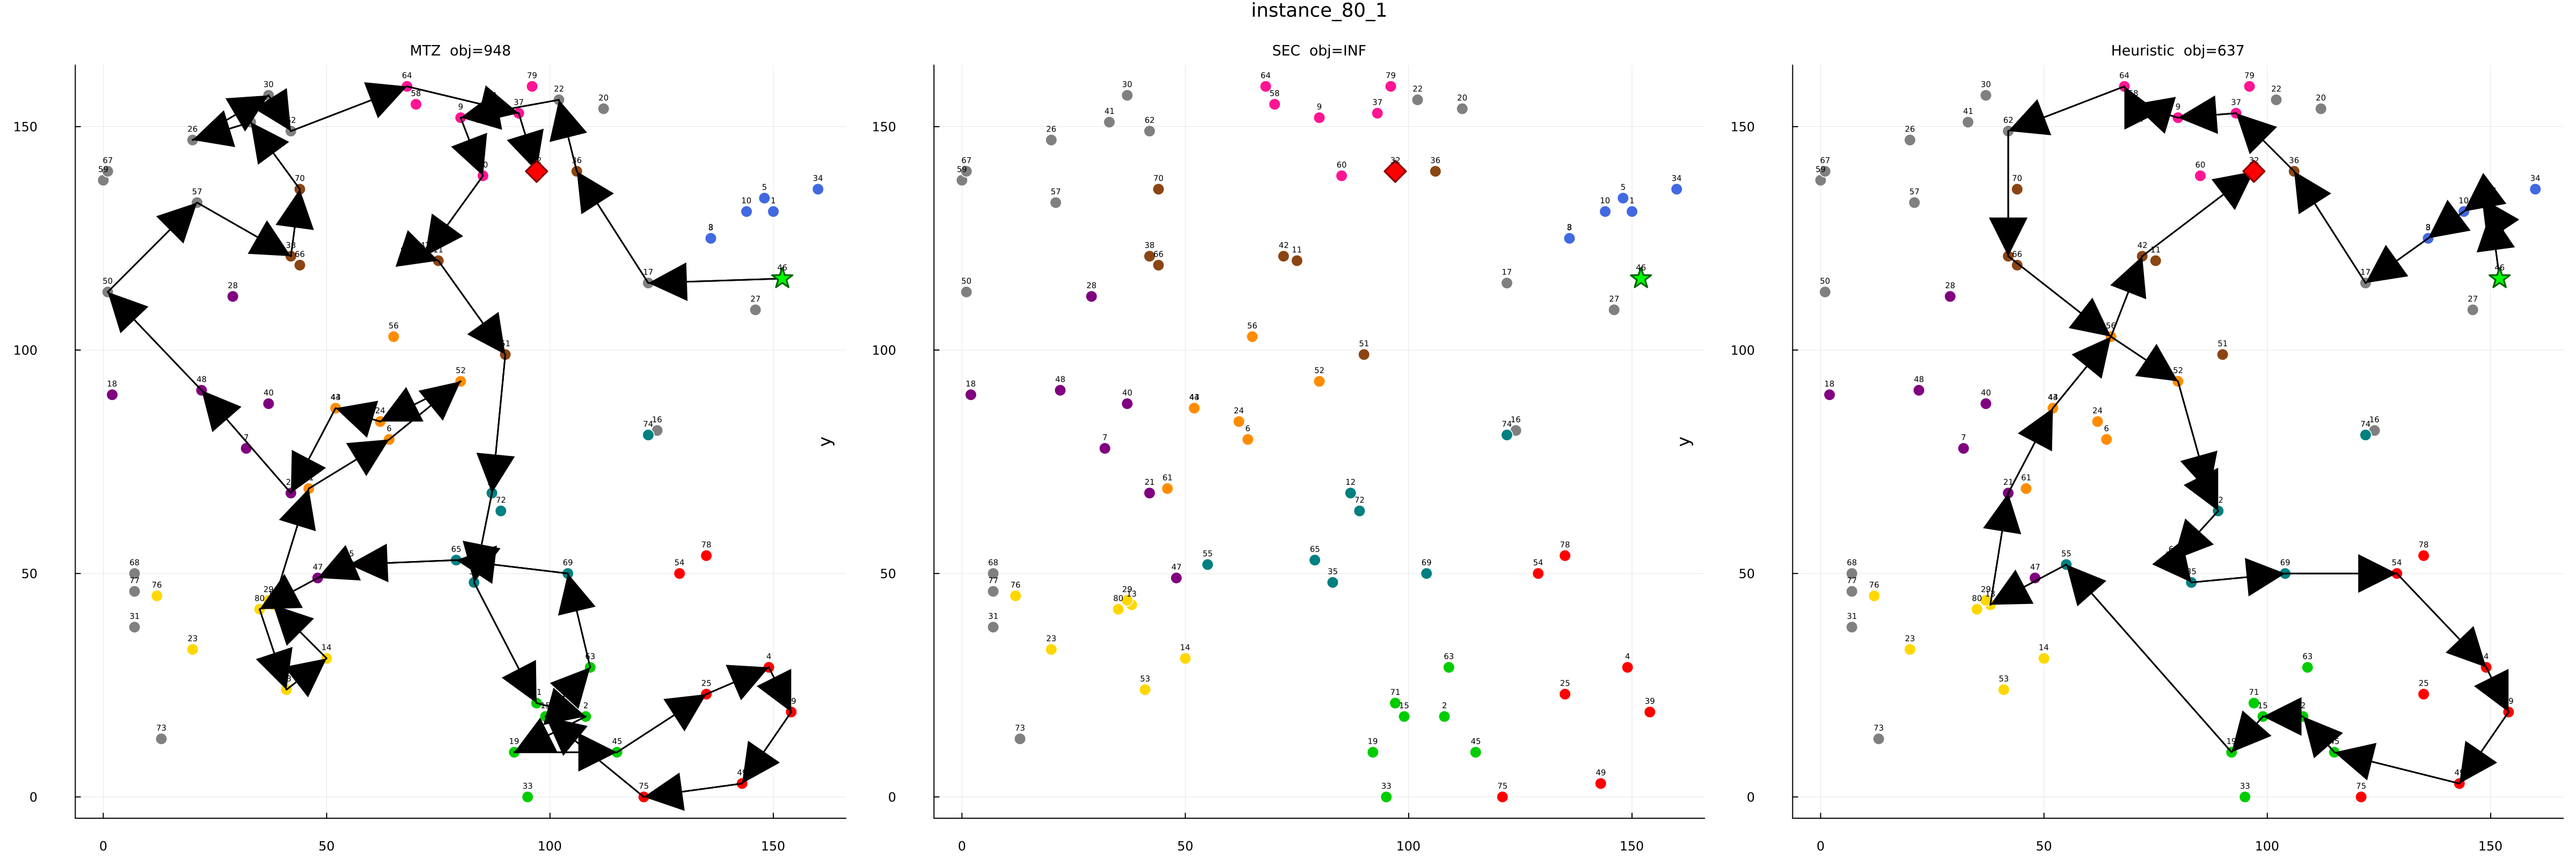
\includegraphics[width=\textwidth]{instance_80_1_results.png}
\end{column}
\end{columns}

\end{frame}

% ================================================================
\begin{frame}{Results --- Custom Instances Summary}

\renewcommand{\arraystretch}{1.18}
\small
\begin{center}
\begin{tabular}{lrrrrrr}
\toprule
\textbf{Instance} & \textbf{$n$} & \textbf{MTZ obj.} & \textbf{MTZ nodes} & \textbf{SEC nodes} & \textbf{Heuristic} & \textbf{Gap} \\
\midrule
\hrow \texttt{20\_1} & 20 & 124 (opt.) & 115\,901 & 177 & 138 & $+11.3\%$ \\
\texttt{20\_2} & 20 & 104 (opt.) & 1\,495   & 224 & 119 & $+14.4\%$ \\
\hrow \texttt{20\_3} & 20 & 104 (opt.) & 892      & 140 & 117 & $+12.5\%$ \\
\texttt{20\_4} & 20 & 109 (opt.) & 142\,906 & 379 & 118 & $+8.3\%$ \\
\hrow \texttt{30\_1} & 30 & 144 (opt.) & 118\,915 & 1\,100 & 152 & $+5.6\%$ \\
\texttt{50\_1} & 50 & 168 (opt.) & 31\,175  & 901 & invalid & --- \\
\hrow \texttt{70\_1} & 70 & 469 (t.l.) & 32\,330  & 11\,647 & invalid & --- \\
\bottomrule
\end{tabular}
\end{center}

\vspace{4pt}
\small
\begin{itemize}\setlength\itemsep{2pt}
  \item MTZ proved optimal on 5 of 7; SEC on 1 of 7 (\texttt{20\_3} only).
  \item SEC B\&B nodes consistently $10\times$--$376\times$ fewer than MTZ.
  \item Heuristic feasible gaps: $5.6\%$--$14.4\%$ where valid.
\end{itemize}

\end{frame}

% ================================================================
\begin{frame}{Analysis --- MTZ vs.\ SEC}

\begin{block}{\textbf{Theory confirmed: SEC needs far fewer B\&B nodes}}
\small
$$z_{\mathrm{LP}}^{\mathrm{SEC}} \geq z_{\mathrm{LP}}^{\mathrm{MTZ}} \geq z_{\mathrm{ILP}}^*$$
Tighter LP bound $\Rightarrow$ more pruning by bound criterion (Cours 2).
\end{block}

\begin{block}{\textbf{But: iterative implementation is slower than MTZ}}
\small
Re-solving from scratch after each cut batch discards the B\&B tree.\\
Two sources of overhead: (i) root restart loses warm-start information; (ii) 90--134 cuts per instance, each triggering a full re-solve.\\[4pt]
\textcolor{darkred}{\textbf{Key point:}} this is an implementation limitation, not a formulation weakness.\\
Lazy-callback SEC would preserve the tree and outperform MTZ on all but tiny instances.
\end{block}

\begin{block}{\textbf{Connection to CORO lectures}}
\small
\begin{itemize}\setlength\itemsep{1pt}
  \item Cours 1 (LP duality): $z_\mathrm{LP}$ is a valid lower bound, exploited by B\&B.
  \item Cours 2 (B\&B): three pruning criteria --- optimality, bound, infeasibility.
  \item Cours 3 (cutting planes): SEC separation = BFS in $O(n+|A|)$.
  \item Cours 4 (Lagrangian relaxation): relaxing C5 (coverage) could give tighter bounds without SEC overhead.
\end{itemize}
\end{block}

\end{frame}

% ================================================================
\begin{frame}{Analysis --- Heuristic Failure on Sparse Instances}

\begin{columns}[T]
\begin{column}{0.50\textwidth}
\begin{block}{\textbf{Root cause}}
\small
Dijkstra escape returns a multi-hop sub-path, range-feasible by construction.\\[4pt]
When the sub-path passes through an already-visited node, that node is skipped to avoid duplicates.\\[4pt]
This leaves a \textcolor{darkred}{direct connection between two non-adjacent nodes that was never checked for range feasibility}.\\[4pt]
Result: adjacent entries in the path vector exceed $R$.
\end{block}

\begin{block}{\textbf{Fix}}
\small
Restrict Dijkstra to only unvisited intermediate nodes, even if this produces a longer sub-path.
\end{block}
\end{column}

\begin{column}{0.48\textwidth}
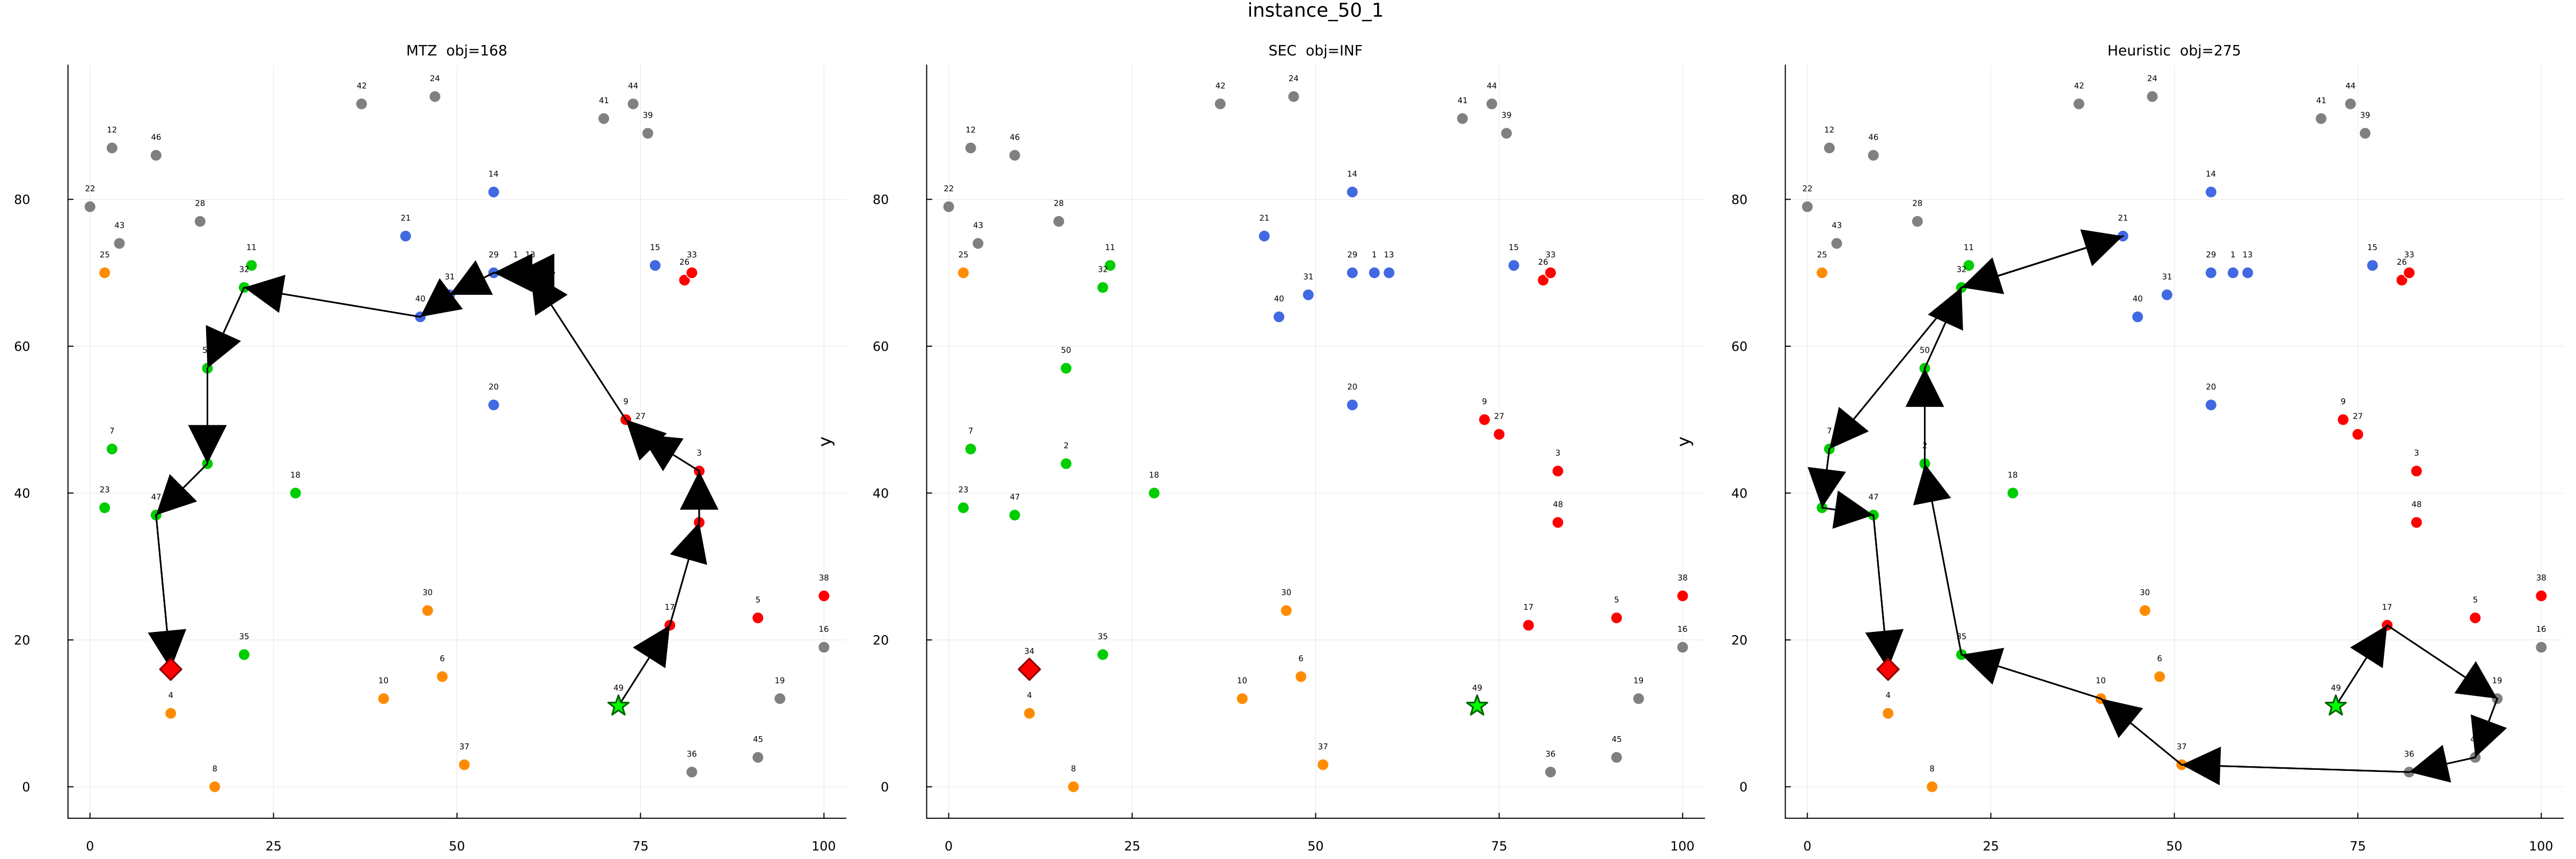
\includegraphics[width=\textwidth]{instance_50_1_results.png}
\vspace{3pt}
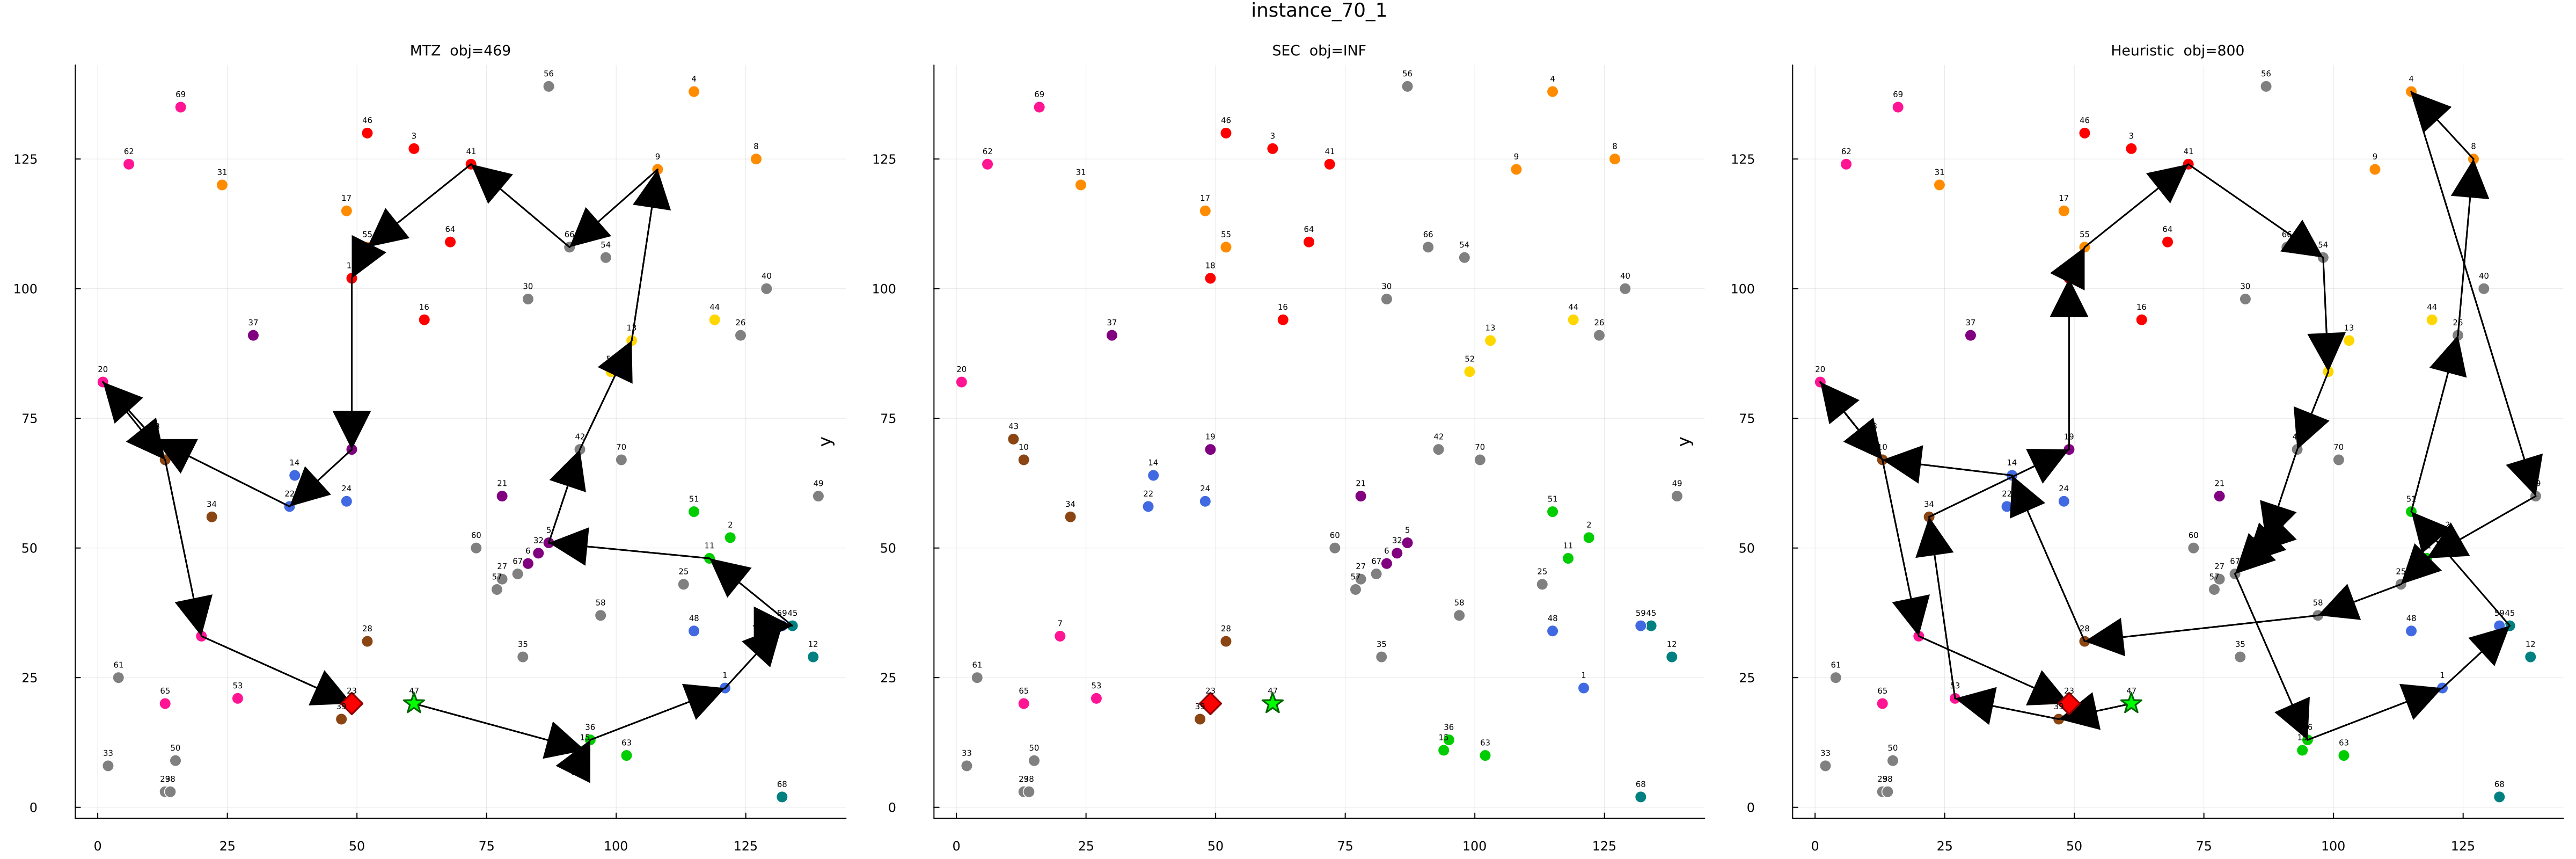
\includegraphics[width=\textwidth]{instance_70_1_results.png}
\end{column}
\end{columns}

\end{frame}

% ================================================================
\begin{frame}{Conclusion}

\begin{block}{\textbf{Summary}}
\small
\begin{itemize}\setlength\itemsep{3pt}
  \item \textbf{MTZ}: practical winner in our implementation --- proved optimal on 7 of 9 instances within 120\,s. Simple, single solve, no iteration overhead.
  \item \textbf{SEC}: theoretically superior LP relaxation confirmed by $10\times$--$376\times$ fewer B\&B nodes. Iterative re-solve overhead prevents it from outperforming MTZ in wall-clock time with our implementation.
  \item \textbf{Heuristic}: $<1$\,ms, gaps of $5$--$14\%$ on feasible instances. Fails on sparse graphs due to range violation in Dijkstra escape.
\end{itemize}
\end{block}

\begin{block}{\textbf{What would improve results}}
\small
\begin{itemize}\setlength\itemsep{3pt}
  \item Implement SEC with \textbf{lazy callbacks} (single B\&B run, no restarts).
  \item Use heuristic solution as \textbf{warm-start incumbent} for both ILP models.
  \item Apply \textbf{Lagrangian relaxation} on region-covering constraints (C5) for a tighter lower bound without SEC overhead (Cours 4).
  \item Fix heuristic Dijkstra escape to preserve range feasibility on sparse graphs.
\end{itemize}
\end{block}

\end{frame}

\end{document}
